\documentclass{beamer}

\usefonttheme{professionalfonts} % using non standard fonts for beamer
\usefonttheme{serif} % default family is serif

\usepackage{hyperref}
%\usepackage{minted}
\usepackage{animate}
\usepackage{graphicx}
\def\Put(#1,#2)#3{\leavevmode\makebox(0,0){\put(#1,#2){#3}}}
\usepackage{colortbl}
\usepackage{tikz}
\usepackage{amssymb}
\usepackage{enumerate}
\usepackage{arydshln}
\usepackage{algorithm}
\usepackage{algpseudocode}

\colorlet{lightred}{red!25}
\colorlet{lightgreen}{green!25}


\newcommand\blfootnote[1]{%

  \begingroup

  \renewcommand\thefootnote{}\footnote{#1}%

  \addtocounter{footnote}{-1}%

  \endgroup

}

\makeatletter

%%%%%%%%%%%%%%%%%%%%%%%%%%%%%% Textclass specific LaTeX commands.

 % this default might be overridden by plain title style

 \newcommand\makebeamertitle{\frame{\maketitle}}%

 % (ERT) argument for the TOC

 \AtBeginDocument{%

   \let\origtableofcontents=\tableofcontents

   \def\tableofcontents{\@ifnextchar[{\origtableofcontents}{\gobbletableofcontents}}

   \def\gobbletableofcontents#1{\origtableofcontents}

 }

%%%%%%%%%%%%%%%%%%%%%%%%%%%%%% User specified LaTeX commands.

\usetheme{Malmoe}

% or ...

\useoutertheme{infolines}

\addtobeamertemplate{headline}{}{\vskip2pt}

\setbeamercovered{transparent}

% or whatever (possibly just delete it)

\makeatother

\begin{document}
\title[PFLOCK report]{PFLOCK Report}
\author[AC]{Andres Calderon}
\institute[Winter'20]{University of California, Riverside}
\makebeamertitle
\newif\iflattersubsect

\AtBeginSection[] {
    \begin{frame}<beamer>
    \frametitle{Outline} 
    \tableofcontents[currentsection]  
    \end{frame}
    \lattersubsectfalse
}

\AtBeginSubsection[] {
    \begin{frame}<beamer>
    \frametitle{Outline} 
    \tableofcontents[currentsubsection]  
    \end{frame}
}

\begin{frame}{Experiment settings...}
    \begin{itemize}
        \item LA\_50K dataset, time instant 320, 50419 points.
        \item $\mu=3$, $\varepsilon$ between 15 and 45.
        \item 12 executors, 9 cores each (108 cores total).
        \item Average time of 3 runs.
        \item Varying values for partitions in quadtree (1 to 4 times number of available cores).
        \item Varying values for paralleism (1 to 4 times number of available cores).
    \end{itemize}
\end{frame}

\begin{frame}{Partitions in quadtre and epsilon...}
    \begin{figure}
        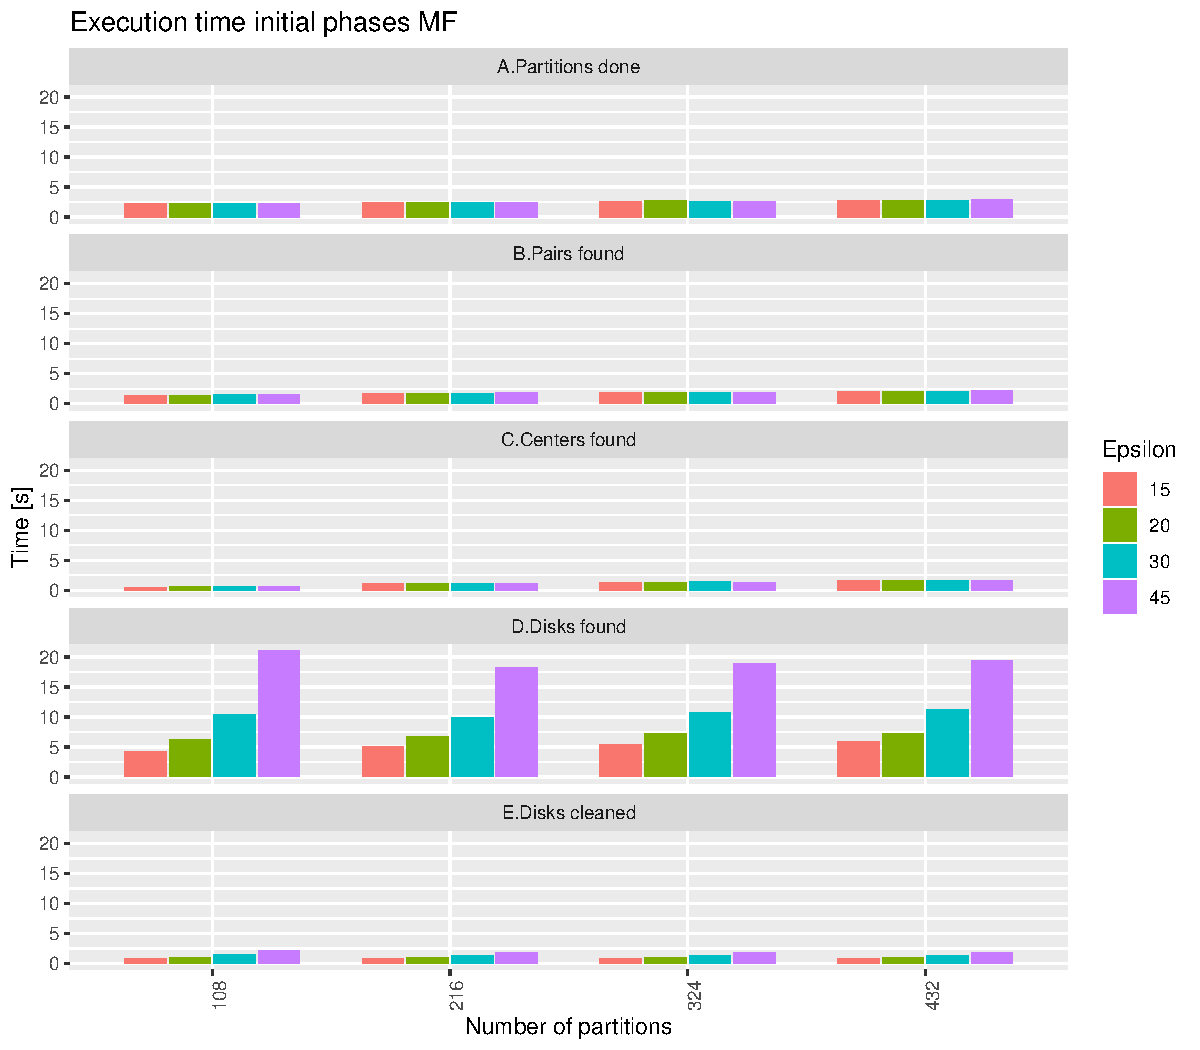
\includegraphics[width=0.75\textwidth]{figures/PartitionTimeEpsilonPhase}
    \end{figure}
\end{frame}

\begin{frame}{Partitions in quadtre and epsilon...}
    \begin{figure}
        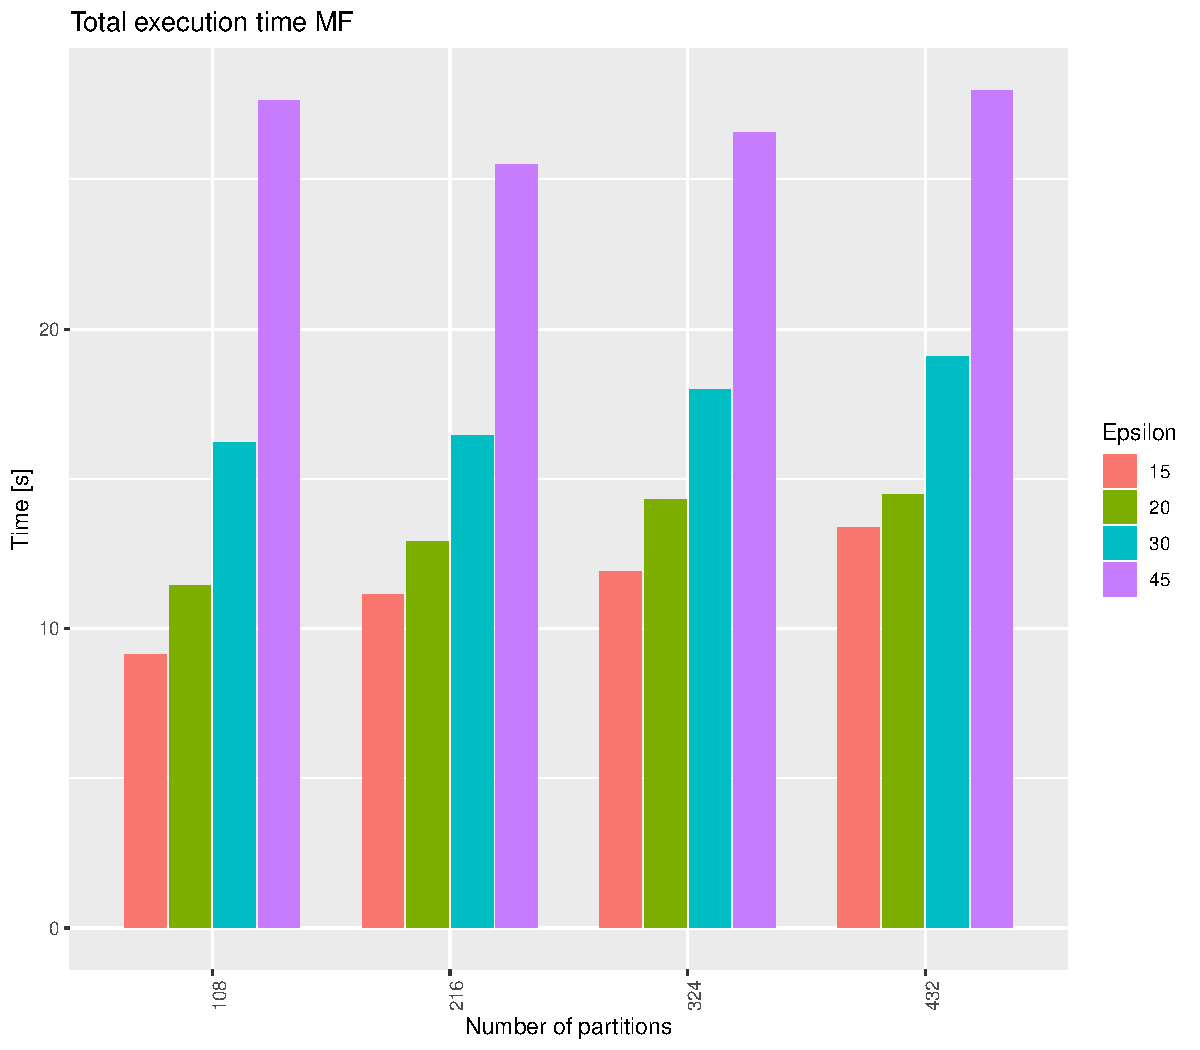
\includegraphics[width=0.75\textwidth]{figures/PartitionTimeEpsilonPhaseTotal}
    \end{figure}
\end{frame}

\begin{frame}{Parallelism...}
    \begin{figure}
        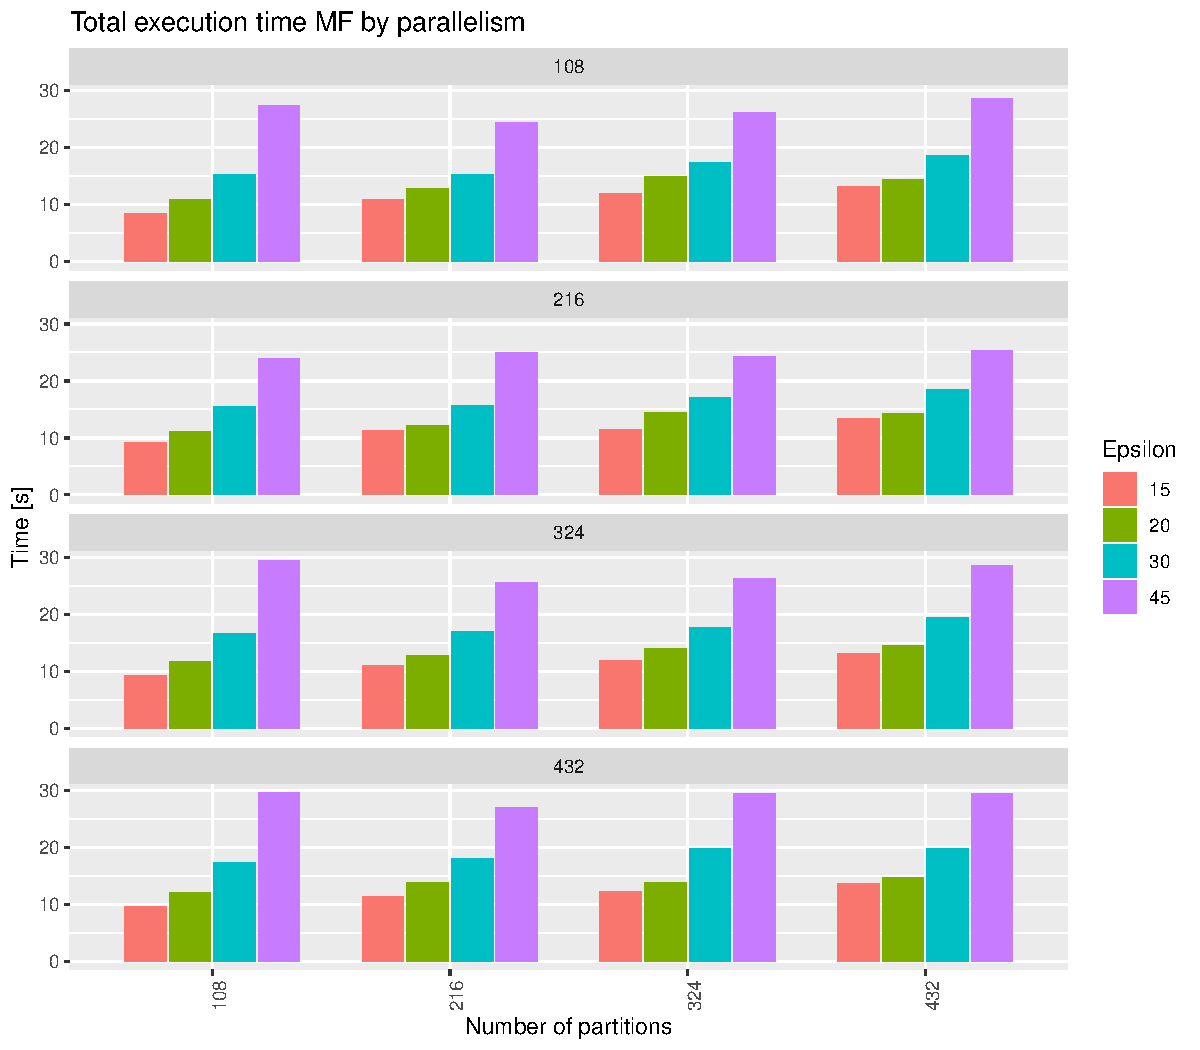
\includegraphics[width=0.75\textwidth]{figures/Parallelism}
    \end{figure}
\end{frame}

\begin{frame}{An issue with repartition between Spark stages...}
    \begin{figure}
        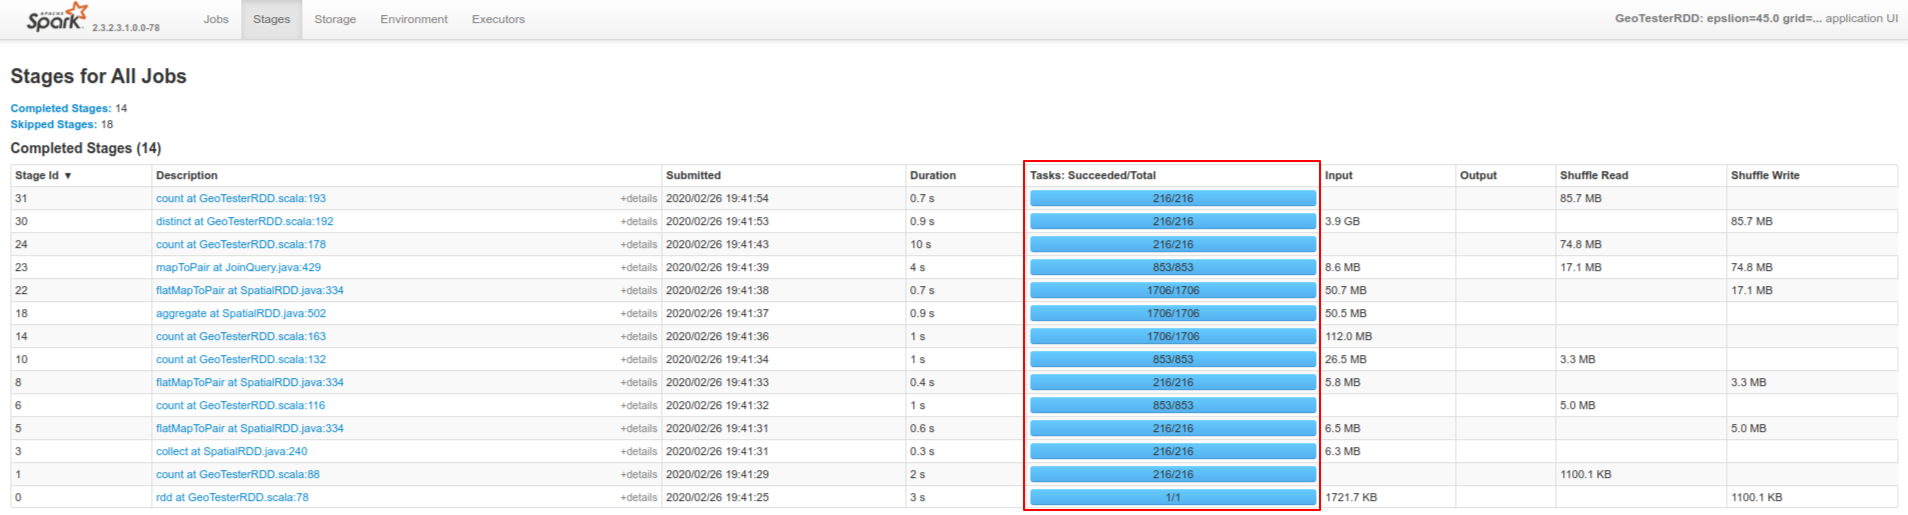
\includegraphics[width=\textwidth]{figures/SparkStages}
    \end{figure}
\end{frame}

\begin{frame}{Task summary...}
    \begin{figure}
        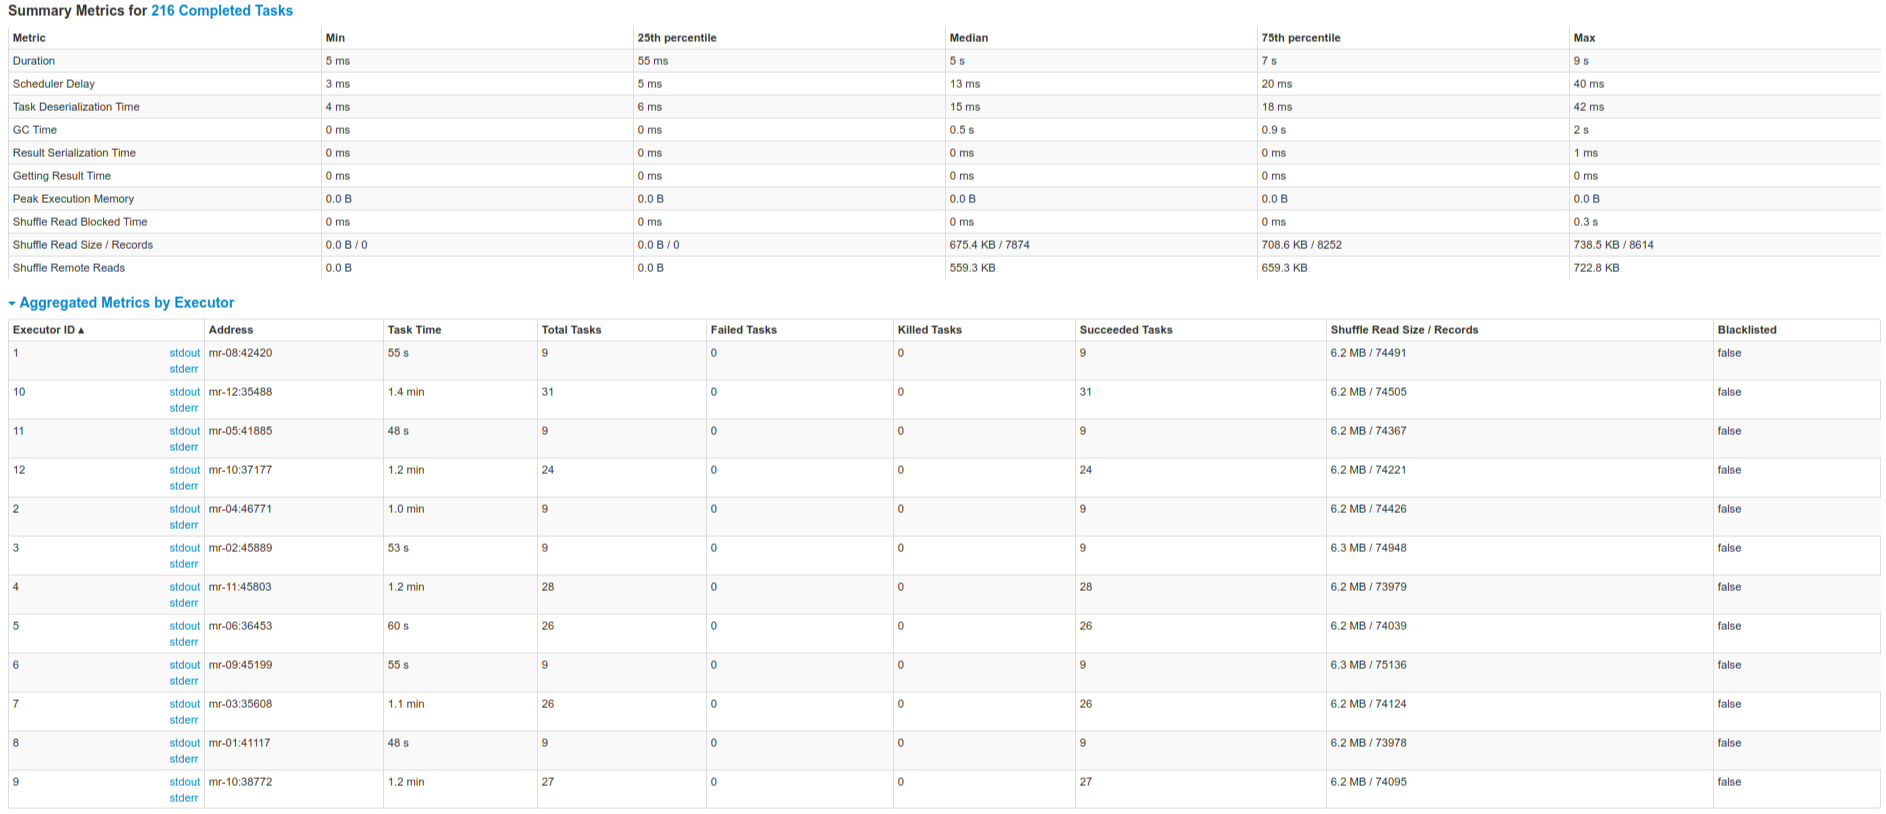
\includegraphics[width=\textwidth]{figures/TaskSummary}
    \end{figure}
    \blfootnote{\tiny Full task info at \url{http://www.cs.ucr.edu/~acald013/public/tmp/geotester1.html}}
\end{frame}

\end{document}
